\documentclass[1p]{elsarticle_modified}
%\bibliographystyle{elsarticle-num}

%\usepackage[colorlinks]{hyperref}
%\usepackage{abbrmath_seonhwa} %\Abb, \Ascr, \Acal ,\Abf, \Afrak
\usepackage{amsfonts}
\usepackage{amssymb}
\usepackage{amsmath}
\usepackage{amsthm}
\usepackage{scalefnt}
\usepackage{amsbsy}
\usepackage{kotex}
\usepackage{caption}
\usepackage{subfig}
\usepackage{color}
\usepackage{graphicx}
\usepackage{xcolor} %% white, black, red, green, blue, cyan, magenta, yellow
\usepackage{float}
\usepackage{setspace}
\usepackage{hyperref}

\usepackage{tikz}
\usetikzlibrary{arrows}

\usepackage{multirow}
\usepackage{array} % fixed length table
\usepackage{hhline}

%%%%%%%%%%%%%%%%%%%%%
\makeatletter
\renewcommand*\env@matrix[1][\arraystretch]{%
	\edef\arraystretch{#1}%
	\hskip -\arraycolsep
	\let\@ifnextchar\new@ifnextchar
	\array{*\c@MaxMatrixCols c}}
\makeatother %https://tex.stackexchange.com/questions/14071/how-can-i-increase-the-line-spacing-in-a-matrix
%%%%%%%%%%%%%%%

\usepackage[normalem]{ulem}

\newcommand{\msout}[1]{\ifmmode\text{\sout{\ensuremath{#1}}}\else\sout{#1}\fi}
%SOURCE: \msout is \stkout macro in https://tex.stackexchange.com/questions/20609/strikeout-in-math-mode

\newcommand{\cancel}[1]{
	\ifmmode
	{\color{red}\msout{#1}}
	\else
	{\color{red}\sout{#1}}
	\fi
}

\newcommand{\add}[1]{
	{\color{blue}\uwave{#1}}
}

\newcommand{\replace}[2]{
	\ifmmode
	{\color{red}\msout{#1}}{\color{blue}\uwave{#2}}
	\else
	{\color{red}\sout{#1}}{\color{blue}\uwave{#2}}
	\fi
}

\newcommand{\Sol}{\mathcal{S}} %segment
\newcommand{\D}{D} %diagram
\newcommand{\A}{\mathcal{A}} %arc


%%%%%%%%%%%%%%%%%%%%%%%%%%%%%5 test

\def\sl{\operatorname{\textup{SL}}(2,\Cbb)}
\def\psl{\operatorname{\textup{PSL}}(2,\Cbb)}
\def\quan{\mkern 1mu \triangleright \mkern 1mu}

\theoremstyle{definition}
\newtheorem{thm}{Theorem}[section]
\newtheorem{prop}[thm]{Proposition}
\newtheorem{lem}[thm]{Lemma}
\newtheorem{ques}[thm]{Question}
\newtheorem{cor}[thm]{Corollary}
\newtheorem{defn}[thm]{Definition}
\newtheorem{exam}[thm]{Example}
\newtheorem{rmk}[thm]{Remark}
\newtheorem{alg}[thm]{Algorithm}

\newcommand{\I}{\sqrt{-1}}
\begin{document}

%\begin{frontmatter}
%
%\title{Boundary parabolic representations of knots up to 8 crossings}
%
%%% Group authors per affiliation:
%\author{Yunhi Cho} 
%\address{Department of Mathematics, University of Seoul, Seoul, Korea}
%\ead{yhcho@uos.ac.kr}
%
%
%\author{Seonhwa Kim} %\fnref{s_kim}}
%\address{Center for Geometry and Physics, Institute for Basic Science, Pohang, 37673, Korea}
%\ead{ryeona17@ibs.re.kr}
%
%\author{Hyuk Kim}
%\address{Department of Mathematical Sciences, Seoul National University, Seoul 08826, Korea}
%\ead{hyukkim@snu.ac.kr}
%
%\author{Seokbeom Yoon}
%\address{Department of Mathematical Sciences, Seoul National University, Seoul, 08826,  Korea}
%\ead{sbyoon15@snu.ac.kr}
%
%\begin{abstract}
%We find all boundary parabolic representation of knots up to 8 crossings.
%
%\end{abstract}
%\begin{keyword}
%    \MSC[2010] 57M25 
%\end{keyword}
%
%\end{frontmatter}

%\linenumbers
%\tableofcontents
%
\newcommand\colored[1]{\textcolor{white}{\rule[-0.35ex]{0.8em}{1.4ex}}\kern-0.8em\color{red} #1}%
%\newcommand\colored[1]{\textcolor{white}{ #1}\kern-2.17ex	\textcolor{white}{ #1}\kern-1.81ex	\textcolor{white}{ #1}\kern-2.15ex\color{red}#1	}

{\Large $\underline{12n_{0239}~(K12n_{0239})}$}

\setlength{\tabcolsep}{10pt}
\renewcommand{\arraystretch}{1.6}
\vspace{1cm}\begin{tabular}{m{100pt}>{\centering\arraybackslash}m{274pt}}
\multirow{5}{120pt}{
	\centering
	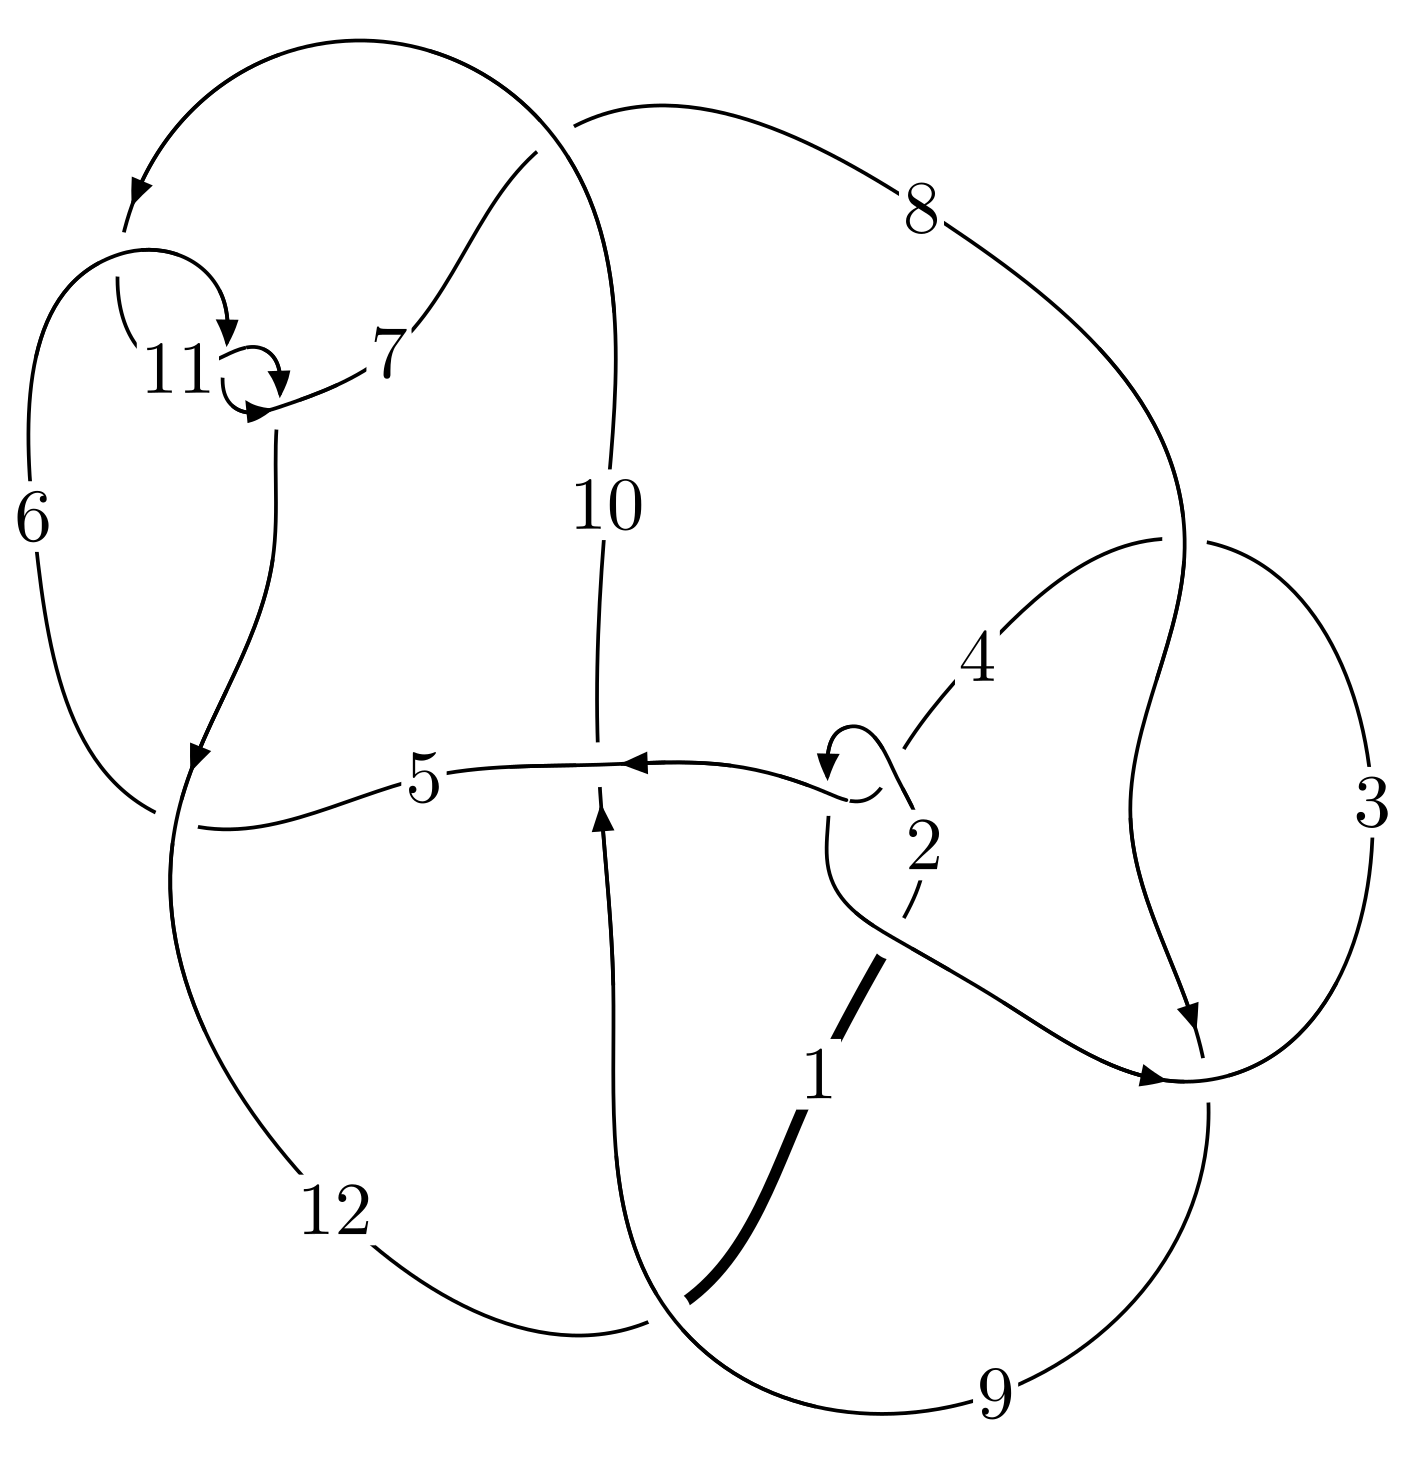
\includegraphics[width=112pt]{../../../GIT/diagram.site/Diagrams/png/2328_12n_0239.png}\\
\ \ \ A knot diagram\footnotemark}&
\allowdisplaybreaks
\textbf{Linearized knot diagam} \\
\cline{2-2}
 &
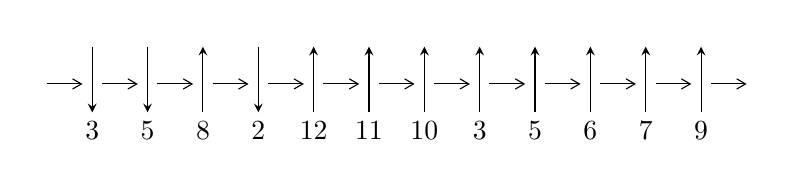
\begin{tikzpicture}[x=20pt, y=17pt]
	% nodes
	\node (C0) at (0, 0) {};
	\node (C1) at (1, 0) {};
	\node (C1U) at (1, +1) {};
	\node (C1D) at (1, -1) {3};

	\node (C2) at (2, 0) {};
	\node (C2U) at (2, +1) {};
	\node (C2D) at (2, -1) {5};

	\node (C3) at (3, 0) {};
	\node (C3U) at (3, +1) {};
	\node (C3D) at (3, -1) {8};

	\node (C4) at (4, 0) {};
	\node (C4U) at (4, +1) {};
	\node (C4D) at (4, -1) {2};

	\node (C5) at (5, 0) {};
	\node (C5U) at (5, +1) {};
	\node (C5D) at (5, -1) {12};

	\node (C6) at (6, 0) {};
	\node (C6U) at (6, +1) {};
	\node (C6D) at (6, -1) {11};

	\node (C7) at (7, 0) {};
	\node (C7U) at (7, +1) {};
	\node (C7D) at (7, -1) {10};

	\node (C8) at (8, 0) {};
	\node (C8U) at (8, +1) {};
	\node (C8D) at (8, -1) {3};

	\node (C9) at (9, 0) {};
	\node (C9U) at (9, +1) {};
	\node (C9D) at (9, -1) {5};

	\node (C10) at (10, 0) {};
	\node (C10U) at (10, +1) {};
	\node (C10D) at (10, -1) {6};

	\node (C11) at (11, 0) {};
	\node (C11U) at (11, +1) {};
	\node (C11D) at (11, -1) {7};

	\node (C12) at (12, 0) {};
	\node (C12U) at (12, +1) {};
	\node (C12D) at (12, -1) {9};
	\node (C13) at (13, 0) {};

	% arrows
	\draw[->,>={angle 60}]
	(C0) edge (C1) (C1) edge (C2) (C2) edge (C3) (C3) edge (C4) (C4) edge (C5) (C5) edge (C6) (C6) edge (C7) (C7) edge (C8) (C8) edge (C9) (C9) edge (C10) (C10) edge (C11) (C11) edge (C12) (C12) edge (C13) ;	\draw[->,>=stealth]
	(C1U) edge (C1D) (C2U) edge (C2D) (C3D) edge (C3U) (C4U) edge (C4D) (C5D) edge (C5U) (C6D) edge (C6U) (C7D) edge (C7U) (C8D) edge (C8U) (C9D) edge (C9U) (C10D) edge (C10U) (C11D) edge (C11U) (C12D) edge (C12U) ;
	\end{tikzpicture} \\
\hhline{~~} \\& 
\textbf{Solving Sequence} \\ \cline{2-2} 
 &
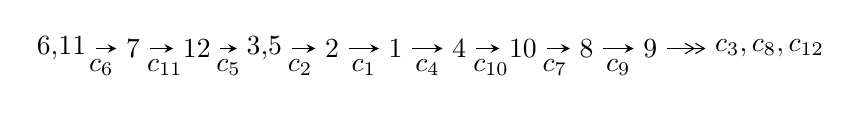
\begin{tikzpicture}[x=23pt, y=7pt]
	% node
	\node (A0) at (-1/8, 0) {6,11};
	\node (A1) at (1, 0) {7};
	\node (A2) at (2, 0) {12};
	\node (A3) at (49/16, 0) {3,5};
	\node (A4) at (33/8, 0) {2};
	\node (A5) at (41/8, 0) {1};
	\node (A6) at (49/8, 0) {4};
	\node (A7) at (57/8, 0) {10};
	\node (A8) at (65/8, 0) {8};
	\node (A9) at (73/8, 0) {9};
	\node (C1) at (1/2, -1) {$c_{6}$};
	\node (C2) at (3/2, -1) {$c_{11}$};
	\node (C3) at (5/2, -1) {$c_{5}$};
	\node (C4) at (29/8, -1) {$c_{2}$};
	\node (C5) at (37/8, -1) {$c_{1}$};
	\node (C6) at (45/8, -1) {$c_{4}$};
	\node (C7) at (53/8, -1) {$c_{10}$};
	\node (C8) at (61/8, -1) {$c_{7}$};
	\node (C9) at (69/8, -1) {$c_{9}$};
	\node (A10) at (11, 0) {$c_{3},c_{8},c_{12}$};

	% edge
	\draw[->,>=stealth]	
	(A0) edge (A1) (A1) edge (A2) (A2) edge (A3) (A3) edge (A4) (A4) edge (A5) (A5) edge (A6) (A6) edge (A7) (A7) edge (A8) (A8) edge (A9) ;
	\draw[->>,>={angle 60}]	
	(A9) edge (A10);
\end{tikzpicture} \\ 

\end{tabular} \\

\footnotetext{
The image of knot diagram is generated by the software ``\textbf{Draw programme}" developed by Andrew Bartholomew(\url{http://www.layer8.co.uk/maths/draw/index.htm\#Running-draw}), where we modified some parts for our purpose(\url{https://github.com/CATsTAILs/LinksPainter}).
}\phantom \\ \newline 
\centering \textbf{Ideals for irreducible components\footnotemark of $X_{\text{par}}$} 
 
\begin{align*}
I^u_{1}&=\langle 
- u^{28}- u^{27}+\cdots+b+u,\;3 u^{28}+3 u^{27}+\cdots+a+1,\;u^{29}+2 u^{28}+\cdots- u+1\rangle \\
I^u_{2}&=\langle 
- u^3+b+u+1,\;- u^6+3 u^4+u^3-2 u^2+a- u-2,\;u^8- u^7-3 u^6+2 u^5+3 u^4-2 u-1\rangle \\
\\
\end{align*}
\raggedright * 2 irreducible components of $\dim_{\mathbb{C}}=0$, with total 37 representations.\\
\footnotetext{All coefficients of polynomials are rational numbers. But the coefficients are sometimes approximated in decimal forms when there is not enough margin.}
\newpage
\renewcommand{\arraystretch}{1}
\centering \section*{I. $I^u_{1}= \langle - u^{28}- u^{27}+\cdots+b+u,\;3 u^{28}+3 u^{27}+\cdots+a+1,\;u^{29}+2 u^{28}+\cdots- u+1 \rangle$}
\flushleft \textbf{(i) Arc colorings}\\
\begin{tabular}{m{7pt} m{180pt} m{7pt} m{180pt} }
\flushright $a_{6}=$&$\begin{pmatrix}1\\0\end{pmatrix}$ \\
\flushright $a_{11}=$&$\begin{pmatrix}0\\u\end{pmatrix}$ \\
\flushright $a_{7}=$&$\begin{pmatrix}1\\- u^2\end{pmatrix}$ \\
\flushright $a_{12}=$&$\begin{pmatrix}u\\- u^3+u\end{pmatrix}$ \\
\flushright $a_{3}=$&$\begin{pmatrix}-3 u^{28}-3 u^{27}+\cdots- u-1\\u^{28}+u^{27}+\cdots+6 u^2- u\end{pmatrix}$ \\
\flushright $a_{5}=$&$\begin{pmatrix}- u^4+u^2+1\\u^6-2 u^4+u^2\end{pmatrix}$ \\
\flushright $a_{2}=$&$\begin{pmatrix}-2 u^{28}-2 u^{27}+\cdots-3 u-1\\u^{28}+u^{27}+\cdots+5 u^2- u\end{pmatrix}$ \\
\flushright $a_{1}=$&$\begin{pmatrix}- u^{21}+8 u^{19}+\cdots-6 u^3- u\\u^{23}-9 u^{21}+\cdots+4 u^3- u\end{pmatrix}$ \\
\flushright $a_{4}=$&$\begin{pmatrix}- u^{28}- u^{27}+\cdots-5 u^2-3 u\\u^{28}+u^{27}+\cdots+8 u^3+5 u^2\end{pmatrix}$ \\
\flushright $a_{10}=$&$\begin{pmatrix}- u\\u\end{pmatrix}$ \\
\flushright $a_{8}=$&$\begin{pmatrix}- u^4+u^2+1\\u^4-2 u^2\end{pmatrix}$ \\
\flushright $a_{9}=$&$\begin{pmatrix}u^{11}-4 u^9+4 u^7+2 u^5-3 u^3-2 u\\- u^{13}+5 u^{11}-9 u^9+6 u^7- u^3+u\end{pmatrix}$\\&\end{tabular}
\flushleft \textbf{(ii) Obstruction class $= -1$}\\~\\
\flushleft \textbf{(iii) Cusp Shapes $= -5 u^{28}-4 u^{27}+53 u^{26}+33 u^{25}-247 u^{24}-102 u^{23}+634 u^{22}+96 u^{21}-879 u^{20}+214 u^{19}+362 u^{18}-658 u^{17}+771 u^{16}+486 u^{15}-1175 u^{14}+371 u^{13}+217 u^{12}-670 u^{11}+671 u^{10}-12 u^9-364 u^8+380 u^7-164 u^6-26 u^5+109 u^4-112 u^3+24 u^2-15 u-1$}\\~\\
\newpage\renewcommand{\arraystretch}{1}
\flushleft \textbf{(iv) u-Polynomials at the component}\newline \\
\begin{tabular}{m{50pt}|m{274pt}}
Crossings & \hspace{64pt}u-Polynomials at each crossing \\
\hline $$\begin{aligned}c_{1}\end{aligned}$$&$\begin{aligned}
&u^{29}+45 u^{28}+\cdots+63 u+1
\end{aligned}$\\
\hline $$\begin{aligned}c_{2},c_{4}\end{aligned}$$&$\begin{aligned}
&u^{29}-9 u^{28}+\cdots-15 u+1
\end{aligned}$\\
\hline $$\begin{aligned}c_{3},c_{8}\end{aligned}$$&$\begin{aligned}
&u^{29}+u^{28}+\cdots-640 u+256
\end{aligned}$\\
\hline $$\begin{aligned}c_{5},c_{7}\end{aligned}$$&$\begin{aligned}
&u^{29}+6 u^{28}+\cdots-27 u-7
\end{aligned}$\\
\hline $$\begin{aligned}c_{6},c_{10},c_{11}\end{aligned}$$&$\begin{aligned}
&u^{29}-2 u^{28}+\cdots- u-1
\end{aligned}$\\
\hline $$\begin{aligned}c_{9}\end{aligned}$$&$\begin{aligned}
&u^{29}+2 u^{28}+\cdots+847 u-505
\end{aligned}$\\
\hline $$\begin{aligned}c_{12}\end{aligned}$$&$\begin{aligned}
&u^{29}+30 u^{27}+\cdots- u+1
\end{aligned}$\\
\hline
\end{tabular}\\~\\
\newpage\renewcommand{\arraystretch}{1}
\flushleft \textbf{(v) Riley Polynomials at the component}\newline \\
\begin{tabular}{m{50pt}|m{274pt}}
Crossings & \hspace{64pt}Riley Polynomials at each crossing \\
\hline $$\begin{aligned}c_{1}\end{aligned}$$&$\begin{aligned}
&y^{29}-113 y^{28}+\cdots+3195 y-1
\end{aligned}$\\
\hline $$\begin{aligned}c_{2},c_{4}\end{aligned}$$&$\begin{aligned}
&y^{29}-45 y^{28}+\cdots+63 y-1
\end{aligned}$\\
\hline $$\begin{aligned}c_{3},c_{8}\end{aligned}$$&$\begin{aligned}
&y^{29}+51 y^{28}+\cdots+835584 y-65536
\end{aligned}$\\
\hline $$\begin{aligned}c_{5},c_{7}\end{aligned}$$&$\begin{aligned}
&y^{29}+24 y^{28}+\cdots+239 y-49
\end{aligned}$\\
\hline $$\begin{aligned}c_{6},c_{10},c_{11}\end{aligned}$$&$\begin{aligned}
&y^{29}-24 y^{28}+\cdots- y-1
\end{aligned}$\\
\hline $$\begin{aligned}c_{9}\end{aligned}$$&$\begin{aligned}
&y^{29}+24 y^{28}+\cdots-2572161 y-255025
\end{aligned}$\\
\hline $$\begin{aligned}c_{12}\end{aligned}$$&$\begin{aligned}
&y^{29}+60 y^{28}+\cdots- y-1
\end{aligned}$\\
\hline
\end{tabular}\\~\\
\newpage\flushleft \textbf{(vi) Complex Volumes and Cusp Shapes}
$$\begin{array}{c|c|c}  
\text{Solutions to }I^u_{1}& \I (\text{vol} + \sqrt{-1}CS) & \text{Cusp shape}\\
 \hline 
\begin{aligned}
u &= \phantom{-}0.116211 + 0.866176 I \\
a &= \phantom{-}0.518979 - 0.390879 I \\
b &= \phantom{-}0.83718 - 3.00348 I\end{aligned}
 & -18.1545 + 6.4457 I & -0.28264 - 3.13315 I \\ \hline\begin{aligned}
u &= \phantom{-}0.116211 - 0.866176 I \\
a &= \phantom{-}0.518979 + 0.390879 I \\
b &= \phantom{-}0.83718 + 3.00348 I\end{aligned}
 & -18.1545 - 6.4457 I & -0.28264 + 3.13315 I \\ \hline\begin{aligned}
u &= \phantom{-}0.025688 + 0.825088 I \\
a &= -0.594569 + 0.459352 I \\
b &= -0.23014 + 2.32002 I\end{aligned}
 & -6.93251 + 1.75256 I & -0.94314 - 1.34488 I \\ \hline\begin{aligned}
u &= \phantom{-}0.025688 - 0.825088 I \\
a &= -0.594569 - 0.459352 I \\
b &= -0.23014 - 2.32002 I\end{aligned}
 & -6.93251 - 1.75256 I & -0.94314 + 1.34488 I \\ \hline\begin{aligned}
u &= \phantom{-}1.19941\phantom{ +0.000000I} \\
a &= \phantom{-}2.02803\phantom{ +0.000000I} \\
b &= -1.96066\phantom{ +0.000000I}\end{aligned}
 & \phantom{-}0.978770\phantom{ +0.000000I} & \phantom{-}8.30090\phantom{ +0.000000I} \\ \hline\begin{aligned}
u &= \phantom{-}1.149060 + 0.431164 I \\
a &= -2.80477 - 0.74741 I \\
b &= \phantom{-}1.17842 + 2.47370 I\end{aligned}
 & -14.9885 - 1.7991 I & \phantom{-}2.59660 - 0.52377 I \\ \hline\begin{aligned}
u &= \phantom{-}1.149060 - 0.431164 I \\
a &= -2.80477 + 0.74741 I \\
b &= \phantom{-}1.17842 - 2.47370 I\end{aligned}
 & -14.9885 + 1.7991 I & \phantom{-}2.59660 + 0.52377 I \\ \hline\begin{aligned}
u &= -0.078085 + 0.755576 I \\
a &= \phantom{-}0.230600 - 0.278548 I \\
b &= -0.073065 - 0.703159 I\end{aligned}
 & -2.53613 - 2.06791 I & \phantom{-}5.52324 + 3.00073 I \\ \hline\begin{aligned}
u &= -0.078085 - 0.755576 I \\
a &= \phantom{-}0.230600 + 0.278548 I \\
b &= -0.073065 + 0.703159 I\end{aligned}
 & -2.53613 + 2.06791 I & \phantom{-}5.52324 - 3.00073 I \\ \hline\begin{aligned}
u &= -1.215610 + 0.296484 I \\
a &= \phantom{-}0.992404 - 0.146386 I \\
b &= -0.306342 + 0.431513 I\end{aligned}
 & \phantom{-}0.91968 - 1.73508 I & \phantom{-}8.51016 + 0.61510 I\\
 \hline 
 \end{array}$$\newpage$$\begin{array}{c|c|c}  
\text{Solutions to }I^u_{1}& \I (\text{vol} + \sqrt{-1}CS) & \text{Cusp shape}\\
 \hline 
\begin{aligned}
u &= -1.215610 - 0.296484 I \\
a &= \phantom{-}0.992404 + 0.146386 I \\
b &= -0.306342 - 0.431513 I\end{aligned}
 & \phantom{-}0.91968 + 1.73508 I & \phantom{-}8.51016 - 0.61510 I \\ \hline\begin{aligned}
u &= \phantom{-}0.497421 + 0.544735 I \\
a &= -1.52270 + 0.49021 I \\
b &= \phantom{-}0.327073 - 0.572505 I\end{aligned}
 & -12.40890 + 1.96182 I & \phantom{-}2.44090 - 3.22875 I \\ \hline\begin{aligned}
u &= \phantom{-}0.497421 - 0.544735 I \\
a &= -1.52270 - 0.49021 I \\
b &= \phantom{-}0.327073 + 0.572505 I\end{aligned}
 & -12.40890 - 1.96182 I & \phantom{-}2.44090 + 3.22875 I \\ \hline\begin{aligned}
u &= -1.274370 + 0.082675 I \\
a &= \phantom{-}0.269484 + 1.345140 I \\
b &= \phantom{-}0.022151 - 0.326489 I\end{aligned}
 & \phantom{-}2.70011 - 2.01756 I & \phantom{-}7.88389 + 3.97312 I \\ \hline\begin{aligned}
u &= -1.274370 - 0.082675 I \\
a &= \phantom{-}0.269484 - 1.345140 I \\
b &= \phantom{-}0.022151 + 0.326489 I\end{aligned}
 & \phantom{-}2.70011 + 2.01756 I & \phantom{-}7.88389 - 3.97312 I \\ \hline\begin{aligned}
u &= \phantom{-}1.248070 + 0.369947 I \\
a &= \phantom{-}1.89588 + 1.19040 I \\
b &= -0.78649 - 2.39370 I\end{aligned}
 & -3.15292 + 2.54446 I & \phantom{-}2.89231 - 2.35754 I \\ \hline\begin{aligned}
u &= \phantom{-}1.248070 - 0.369947 I \\
a &= \phantom{-}1.89588 - 1.19040 I \\
b &= -0.78649 + 2.39370 I\end{aligned}
 & -3.15292 - 2.54446 I & \phantom{-}2.89231 + 2.35754 I \\ \hline\begin{aligned}
u &= -1.289030 + 0.369909 I \\
a &= -2.15007 + 1.65647 I \\
b &= \phantom{-}0.23955 - 2.15882 I\end{aligned}
 & -2.83662 - 6.04967 I & \phantom{-}3.35930 + 4.53104 I \\ \hline\begin{aligned}
u &= -1.289030 - 0.369909 I \\
a &= -2.15007 - 1.65647 I \\
b &= \phantom{-}0.23955 + 2.15882 I\end{aligned}
 & -2.83662 + 6.04967 I & \phantom{-}3.35930 - 4.53104 I \\ \hline\begin{aligned}
u &= \phantom{-}1.35324\phantom{ +0.000000I} \\
a &= -0.560180\phantom{ +0.000000I} \\
b &= \phantom{-}0.713936\phantom{ +0.000000I}\end{aligned}
 & \phantom{-}5.98164\phantom{ +0.000000I} & \phantom{-}16.6760\phantom{ +0.000000I}\\
 \hline 
 \end{array}$$\newpage$$\begin{array}{c|c|c}  
\text{Solutions to }I^u_{1}& \I (\text{vol} + \sqrt{-1}CS) & \text{Cusp shape}\\
 \hline 
\begin{aligned}
u &= \phantom{-}1.321100 + 0.324348 I \\
a &= -0.492619 - 0.546231 I \\
b &= \phantom{-}0.144058 + 0.921802 I\end{aligned}
 & \phantom{-}1.85790 + 5.97624 I & \phantom{-}10.99426 - 4.76972 I \\ \hline\begin{aligned}
u &= \phantom{-}1.321100 - 0.324348 I \\
a &= -0.492619 + 0.546231 I \\
b &= \phantom{-}0.144058 - 0.921802 I\end{aligned}
 & \phantom{-}1.85790 - 5.97624 I & \phantom{-}10.99426 + 4.76972 I \\ \hline\begin{aligned}
u &= -1.350820 + 0.384218 I \\
a &= \phantom{-}1.84401 - 2.84917 I \\
b &= \phantom{-}0.46306 + 3.28611 I\end{aligned}
 & -13.5440 - 10.9372 I & \phantom{-}3.78628 + 5.28747 I \\ \hline\begin{aligned}
u &= -1.350820 - 0.384218 I \\
a &= \phantom{-}1.84401 + 2.84917 I \\
b &= \phantom{-}0.46306 - 3.28611 I\end{aligned}
 & -13.5440 + 10.9372 I & \phantom{-}3.78628 - 5.28747 I \\ \hline\begin{aligned}
u &= -1.41186 + 0.13721 I \\
a &= -0.04816 - 1.43092 I \\
b &= -0.645077 + 1.183340 I\end{aligned}
 & -6.30066 - 4.18073 I & \phantom{-}6.94767 + 2.86022 I \\ \hline\begin{aligned}
u &= -1.41186 - 0.13721 I \\
a &= -0.04816 + 1.43092 I \\
b &= -0.645077 - 1.183340 I\end{aligned}
 & -6.30066 + 4.18073 I & \phantom{-}6.94767 - 2.86022 I \\ \hline\begin{aligned}
u &= -0.378524\phantom{ +0.000000I} \\
a &= \phantom{-}0.615391\phantom{ +0.000000I} \\
b &= \phantom{-}0.176038\phantom{ +0.000000I}\end{aligned}
 & \phantom{-}0.641421\phantom{ +0.000000I} & \phantom{-}15.6290\phantom{ +0.000000I} \\ \hline\begin{aligned}
u &= \phantom{-}0.175172 + 0.291603 I \\
a &= \phantom{-}0.31991 - 2.02255 I \\
b &= -0.635045 + 0.442420 I\end{aligned}
 & -1.62334 + 0.70173 I & -1.51173 - 3.13517 I \\ \hline\begin{aligned}
u &= \phantom{-}0.175172 - 0.291603 I \\
a &= \phantom{-}0.31991 + 2.02255 I \\
b &= -0.635045 - 0.442420 I\end{aligned}
 & -1.62334 - 0.70173 I & -1.51173 + 3.13517 I\\
 \hline 
 \end{array}$$\newpage\newpage\renewcommand{\arraystretch}{1}
\centering \section*{II. $I^u_{2}= \langle - u^3+b+u+1,\;- u^6+3 u^4+u^3-2 u^2+a- u-2,\;u^8- u^7-3 u^6+2 u^5+3 u^4-2 u-1 \rangle$}
\flushleft \textbf{(i) Arc colorings}\\
\begin{tabular}{m{7pt} m{180pt} m{7pt} m{180pt} }
\flushright $a_{6}=$&$\begin{pmatrix}1\\0\end{pmatrix}$ \\
\flushright $a_{11}=$&$\begin{pmatrix}0\\u\end{pmatrix}$ \\
\flushright $a_{7}=$&$\begin{pmatrix}1\\- u^2\end{pmatrix}$ \\
\flushright $a_{12}=$&$\begin{pmatrix}u\\- u^3+u\end{pmatrix}$ \\
\flushright $a_{3}=$&$\begin{pmatrix}u^6-3 u^4- u^3+2 u^2+u+2\\u^3- u-1\end{pmatrix}$ \\
\flushright $a_{5}=$&$\begin{pmatrix}- u^4+u^2+1\\u^6-2 u^4+u^2\end{pmatrix}$ \\
\flushright $a_{2}=$&$\begin{pmatrix}u^6-2 u^4- u^3+u^2+u+1\\- u^6+2 u^4+u^3- u^2- u-1\end{pmatrix}$ \\
\flushright $a_{1}=$&$\begin{pmatrix}u^4- u^2-1\\- u^6+2 u^4- u^2\end{pmatrix}$ \\
\flushright $a_{4}=$&$\begin{pmatrix}u^6-3 u^4- u^3+2 u^2+u+2\\u^3- u-1\end{pmatrix}$ \\
\flushright $a_{10}=$&$\begin{pmatrix}- u\\u\end{pmatrix}$ \\
\flushright $a_{8}=$&$\begin{pmatrix}- u^4+u^2+1\\u^4-2 u^2\end{pmatrix}$ \\
\flushright $a_{9}=$&$\begin{pmatrix}- u^4+u^2+1\\u^4-2 u^2\end{pmatrix}$\\&\end{tabular}
\flushleft \textbf{(ii) Obstruction class $= 1$}\\~\\
\flushleft \textbf{(iii) Cusp Shapes $= u^7+2 u^6-2 u^5-8 u^4-3 u^3+7 u^2+8 u+7$}\\~\\
\newpage\renewcommand{\arraystretch}{1}
\flushleft \textbf{(iv) u-Polynomials at the component}\newline \\
\begin{tabular}{m{50pt}|m{274pt}}
Crossings & \hspace{64pt}u-Polynomials at each crossing \\
\hline $$\begin{aligned}c_{1},c_{2}\end{aligned}$$&$\begin{aligned}
&(u-1)^8
\end{aligned}$\\
\hline $$\begin{aligned}c_{3},c_{8}\end{aligned}$$&$\begin{aligned}
&u^8
\end{aligned}$\\
\hline $$\begin{aligned}c_{4}\end{aligned}$$&$\begin{aligned}
&(u+1)^8
\end{aligned}$\\
\hline $$\begin{aligned}c_{5},c_{7}\end{aligned}$$&$\begin{aligned}
&u^8+3 u^7+7 u^6+10 u^5+11 u^4+10 u^3+6 u^2+4 u+1
\end{aligned}$\\
\hline $$\begin{aligned}c_{6}\end{aligned}$$&$\begin{aligned}
&u^8- u^7-3 u^6+2 u^5+3 u^4-2 u-1
\end{aligned}$\\
\hline $$\begin{aligned}c_{9},c_{12}\end{aligned}$$&$\begin{aligned}
&u^8- u^7- u^6+2 u^5+u^4-2 u^3+2 u-1
\end{aligned}$\\
\hline $$\begin{aligned}c_{10},c_{11}\end{aligned}$$&$\begin{aligned}
&u^8+u^7-3 u^6-2 u^5+3 u^4+2 u-1
\end{aligned}$\\
\hline
\end{tabular}\\~\\
\newpage\renewcommand{\arraystretch}{1}
\flushleft \textbf{(v) Riley Polynomials at the component}\newline \\
\begin{tabular}{m{50pt}|m{274pt}}
Crossings & \hspace{64pt}Riley Polynomials at each crossing \\
\hline $$\begin{aligned}c_{1},c_{2},c_{4}\end{aligned}$$&$\begin{aligned}
&(y-1)^8
\end{aligned}$\\
\hline $$\begin{aligned}c_{3},c_{8}\end{aligned}$$&$\begin{aligned}
&y^8
\end{aligned}$\\
\hline $$\begin{aligned}c_{5},c_{7}\end{aligned}$$&$\begin{aligned}
&y^8+5 y^7+11 y^6+6 y^5-17 y^4-34 y^3-22 y^2-4 y+1
\end{aligned}$\\
\hline $$\begin{aligned}c_{6},c_{10},c_{11}\end{aligned}$$&$\begin{aligned}
&y^8-7 y^7+19 y^6-22 y^5+3 y^4+14 y^3-6 y^2-4 y+1
\end{aligned}$\\
\hline $$\begin{aligned}c_{9},c_{12}\end{aligned}$$&$\begin{aligned}
&y^8-3 y^7+7 y^6-10 y^5+11 y^4-10 y^3+6 y^2-4 y+1
\end{aligned}$\\
\hline
\end{tabular}\\~\\
\newpage\flushleft \textbf{(vi) Complex Volumes and Cusp Shapes}
$$\begin{array}{c|c|c}  
\text{Solutions to }I^u_{2}& \I (\text{vol} + \sqrt{-1}CS) & \text{Cusp shape}\\
 \hline 
\begin{aligned}
u &= -1.180120 + 0.268597 I \\
a &= \phantom{-}1.53392 - 0.14090 I \\
b &= -1.20799 + 0.83423 I\end{aligned}
 & -0.604279 - 1.131230 I & \phantom{-}3.90459 + 0.80511 I \\ \hline\begin{aligned}
u &= -1.180120 - 0.268597 I \\
a &= \phantom{-}1.53392 + 0.14090 I \\
b &= -1.20799 - 0.83423 I\end{aligned}
 & -0.604279 + 1.131230 I & \phantom{-}3.90459 - 0.80511 I \\ \hline\begin{aligned}
u &= -0.108090 + 0.747508 I \\
a &= -0.322641 + 0.144481 I \\
b &= -0.711982 - 1.138990 I\end{aligned}
 & -3.80435 - 2.57849 I & -0.21961 + 3.88175 I \\ \hline\begin{aligned}
u &= -0.108090 - 0.747508 I \\
a &= -0.322641 - 0.144481 I \\
b &= -0.711982 + 1.138990 I\end{aligned}
 & -3.80435 + 2.57849 I & -0.21961 - 3.88175 I \\ \hline\begin{aligned}
u &= \phantom{-}1.37100\phantom{ +0.000000I} \\
a &= \phantom{-}0.595007\phantom{ +0.000000I} \\
b &= \phantom{-}0.205997\phantom{ +0.000000I}\end{aligned}
 & \phantom{-}4.85780\phantom{ +0.000000I} & \phantom{-}7.82890\phantom{ +0.000000I} \\ \hline\begin{aligned}
u &= \phantom{-}1.334530 + 0.318930 I \\
a &= -0.47742 - 1.64247 I \\
b &= -0.365014 + 1.352640 I\end{aligned}
 & \phantom{-}0.73474 + 6.44354 I & \phantom{-}4.50908 - 6.04101 I \\ \hline\begin{aligned}
u &= \phantom{-}1.334530 - 0.318930 I \\
a &= -0.47742 + 1.64247 I \\
b &= -0.365014 - 1.352640 I\end{aligned}
 & \phantom{-}0.73474 - 6.44354 I & \phantom{-}4.50908 + 6.04101 I \\ \hline\begin{aligned}
u &= -0.463640\phantom{ +0.000000I} \\
a &= \phantom{-}1.93726\phantom{ +0.000000I} \\
b &= -0.636025\phantom{ +0.000000I}\end{aligned}
 & -0.799899\phantom{ +0.000000I} & \phantom{-}4.78300\phantom{ +0.000000I}\\
 \hline 
 \end{array}$$\newpage
\newpage\renewcommand{\arraystretch}{1}
\centering \section*{ III. u-Polynomials}
\begin{tabular}{m{50pt}|m{274pt}}
Crossings & \hspace{64pt}u-Polynomials at each crossing \\
\hline $$\begin{aligned}c_{1}\end{aligned}$$&$\begin{aligned}
&((u-1)^8)(u^{29}+45 u^{28}+\cdots+63 u+1)
\end{aligned}$\\
\hline $$\begin{aligned}c_{2}\end{aligned}$$&$\begin{aligned}
&((u-1)^8)(u^{29}-9 u^{28}+\cdots-15 u+1)
\end{aligned}$\\
\hline $$\begin{aligned}c_{3},c_{8}\end{aligned}$$&$\begin{aligned}
&u^8(u^{29}+u^{28}+\cdots-640 u+256)
\end{aligned}$\\
\hline $$\begin{aligned}c_{4}\end{aligned}$$&$\begin{aligned}
&((u+1)^8)(u^{29}-9 u^{28}+\cdots-15 u+1)
\end{aligned}$\\
\hline $$\begin{aligned}c_{5},c_{7}\end{aligned}$$&$\begin{aligned}
&(u^8+3 u^7+7 u^6+10 u^5+11 u^4+10 u^3+6 u^2+4 u+1)\\
&\cdot(u^{29}+6 u^{28}+\cdots-27 u-7)
\end{aligned}$\\
\hline $$\begin{aligned}c_{6}\end{aligned}$$&$\begin{aligned}
&(u^8- u^7-3 u^6+2 u^5+3 u^4-2 u-1)(u^{29}-2 u^{28}+\cdots- u-1)
\end{aligned}$\\
\hline $$\begin{aligned}c_{9}\end{aligned}$$&$\begin{aligned}
&(u^8- u^7+\cdots+2 u-1)(u^{29}+2 u^{28}+\cdots+847 u-505)
\end{aligned}$\\
\hline $$\begin{aligned}c_{10},c_{11}\end{aligned}$$&$\begin{aligned}
&(u^8+u^7-3 u^6-2 u^5+3 u^4+2 u-1)(u^{29}-2 u^{28}+\cdots- u-1)
\end{aligned}$\\
\hline $$\begin{aligned}c_{12}\end{aligned}$$&$\begin{aligned}
&(u^8- u^7+\cdots+2 u-1)(u^{29}+30 u^{27}+\cdots- u+1)
\end{aligned}$\\
\hline
\end{tabular}\newpage\renewcommand{\arraystretch}{1}
\centering \section*{ IV. Riley Polynomials}
\begin{tabular}{m{50pt}|m{274pt}}
Crossings & \hspace{64pt}Riley Polynomials at each crossing \\
\hline $$\begin{aligned}c_{1}\end{aligned}$$&$\begin{aligned}
&((y-1)^8)(y^{29}-113 y^{28}+\cdots+3195 y-1)
\end{aligned}$\\
\hline $$\begin{aligned}c_{2},c_{4}\end{aligned}$$&$\begin{aligned}
&((y-1)^8)(y^{29}-45 y^{28}+\cdots+63 y-1)
\end{aligned}$\\
\hline $$\begin{aligned}c_{3},c_{8}\end{aligned}$$&$\begin{aligned}
&y^8(y^{29}+51 y^{28}+\cdots+835584 y-65536)
\end{aligned}$\\
\hline $$\begin{aligned}c_{5},c_{7}\end{aligned}$$&$\begin{aligned}
&(y^8+5 y^7+11 y^6+6 y^5-17 y^4-34 y^3-22 y^2-4 y+1)\\
&\cdot(y^{29}+24 y^{28}+\cdots+239 y-49)
\end{aligned}$\\
\hline $$\begin{aligned}c_{6},c_{10},c_{11}\end{aligned}$$&$\begin{aligned}
&(y^8-7 y^7+19 y^6-22 y^5+3 y^4+14 y^3-6 y^2-4 y+1)\\
&\cdot(y^{29}-24 y^{28}+\cdots- y-1)
\end{aligned}$\\
\hline $$\begin{aligned}c_{9}\end{aligned}$$&$\begin{aligned}
&(y^8-3 y^7+7 y^6-10 y^5+11 y^4-10 y^3+6 y^2-4 y+1)\\
&\cdot(y^{29}+24 y^{28}+\cdots-2572161 y-255025)
\end{aligned}$\\
\hline $$\begin{aligned}c_{12}\end{aligned}$$&$\begin{aligned}
&(y^8-3 y^7+7 y^6-10 y^5+11 y^4-10 y^3+6 y^2-4 y+1)\\
&\cdot(y^{29}+60 y^{28}+\cdots- y-1)
\end{aligned}$\\
\hline
\end{tabular}
\vskip 2pc
\end{document}